\documentclass[12pt]{article}%
\usepackage{amsfonts}
\usepackage{fancyhdr}
\usepackage{comment,hyperref}
\usepackage[a4paper, top=2.5cm, bottom=2.5cm, left=2.2cm, right=2.2cm]%
{geometry}
\usepackage{times}
\usepackage{amsmath}
\usepackage{changepage}
\usepackage{amssymb}
\usepackage{graphicx}%
\setcounter{MaxMatrixCols}{30}
\newtheorem{theorem}{Theorem}
\newtheorem{corollary}[theorem]{Corollary}
\newtheorem{definition}[theorem]{Definition}
\newtheorem{lemma}[theorem]{Lemma}
\newtheorem{proposition}[theorem]{Proposition}
\newenvironment{proof}[1][Proof]{\textbf{#1.} }{\ \rule{0.5em}{0.5em}}
\newcommand{\poly}{\text{poly}}

\newcommand{\disclaimer}{\textbf{These notes may contain errors, and are not intended for use as a primary source.} I have included references at the end of the notes for those who wish detail surrounding skipped steps.}

\begin{document}

\title{COS 597F - Lecture 1} 
\date{September 12th 2018}
\maketitle

\disclaimer
\section{Admin Stuff}
\begin{itemize}
\item Class administration will be pretty light. There will be PSets and they will be graded, but the grading will be less rigorous than in other classes. Depending on how big the class stays, we may use peer grading to give feedback.
\item Website will be up shortly.
\item Everyone taking the class for credit will do a course project/presentation. More details later, but this can either be a presentation of original research, or presentation of a paper related to the course but not covered (or deeper detail that I omitted about a paper). Depending on the size of the class, this may be done in partners.
\item Will ask for scribes for lectures. This is to 1) make the lecture notes better and 2) isolate writing skills for clarity. I will give you my lecture notes and just ask you to touch them up (could be making definitions more formal/clear, fixing bugs, etc.). 
\item You can collaborate with anyone on the homeworks, including the Internet, or sources referenced in lectures.
\item No regularly scheduled office hours. Will use Piazza for administration (please enroll). 
\item Focus of class will be on getting people up to speed for research (with me), but people generally interested in theory should find the class interesting anyway. 
\item I'm going to focus on two classes of major open problems in this area: combinatorial auctions and multi-item auction design. Both have an approximation algorithms flavor. Combinatorial auctions are a bit more algorithmic, and multi-item auctions are a bit more economics-y.
\end{itemize}

\section{Combinatorial Auctions - Introduction}
Consider the following problem: there are $m$ items to be divided among $n$ bidders. Each bidder $i$ has a valuation function $v_i(\cdot)$ which takes as input a subset of $[m]$ and outputs a non-negative real number. The problem we face is the following: how to partition into disjoint sets $S_1,\ldots, S_n$ so as to maximize $\sum_i v_i(S_i)$, called the \emph{welfare}. 

This problem serves as one of the core motivating problems in algorithmic game theory: it is already a natural algorithmic problem without worrying about incentives. But it is also natural to bring in incentives of the bidders: maybe you don't know the bidders' valuation functions, and you have to ask them for information. But the bidders may try to manipulate you into giving them a set they like better. It's currently unclear how we should evaluate an algorithm when incentives matter, and we'll get into this shortly. I bring this up now because the overarching theme of this class of problems is to \textbf{evaluate the guarantees achievable by computationally efficient algorithms without concern for incentives versus those achievable by computationally efficient mechanisms which must further accommodate bidders' incentives}. 

\subsection{Combinatorial Auctions with Incentives}
Let's allow the auctioneer to charge the bidders if she desires. So now a full outcome is a partition of the items along with a price $p_i$ for each bidder $i$. We say that the bidders are \emph{quasi-linear} if their utility is equal to $v_i(S_i) - p_i$ (and they prefer to maximize their utility). We further say that bidders are \emph{risk-neutral} if they prefer to maximize their expected utility. Unless explicitly stated otherwise, all bidders will be quasi-linear and risk-neutral for this entire class. One implication of these assumptions is, for example, that a bidder doesn't care about other items going to specific other bidders. Below are a few natural classes of auctions to consider:

\begin{definition}[Direct Mechanism] An auction is \emph{direct} if it simply asks each bidder to report a valuation function, and each bidder only interacts with the auction by providing this valuation function.
\end{definition}

\begin{definition}[Dominant Strategy Truthful] A direct mechanism is \emph{dominant strategy truthful} if for all bidders $i$, and all valuations $v_i(\cdot)$ that bidder might have, bidder $i$ weakly maximizes her utility by truthfully reporting $v_i(\cdot)$.\footnote{Technically, the definition also requires that for all $v'_i(\cdot)$, there exists some $v_{-i}(\cdot)$ such that bidder $i$ strictly prefers to report $v_i(\cdot)$ over $v'_i(\cdot)$ against $v_{-i}(\cdot)$, but this is almost never proved, and sometimes the requirement is even dropped from the formal definition.}
\end{definition}

\begin{definition}[Indirect Mechanism] An auction is indirect if it is not direct. For instance, it may interact with each bidder multiple times and may not learn any bidder's entire valuation function. For instance, ``everyone raise your hand if you're willing to pay $x$'' and then awarding the item uniformly at random to one of those raising their hand (or uniformly at random if no one does) would be indirect. Or binary searching for a price where only one person raises their hand in this way. Note that we assume each bidder's valuation function stays constant; i.e. doesn't change over time nor in response to other bidder's answers, if public.
\end{definition}

\begin{definition}[Truthful/Ex-Post Nash] We call an indirect auction truthful if it is an ex-post Nash. We will not give the mathematically formalized definition here, but we characterize it as follows: For each bidder $i$, if each other bidder behaves according to some valuation, then no matter what those valuations are, bidder $i$ wants to behave according to their true valuation; i.e. they respond to the auctioneers questions truthfully. We also note that each time the auctioneer interacts with bidder $i$, their questions can be answered knowing $v_i(\cdot)$.
\end{definition}

We'll see some examples illustrating these properties in the remainder of lecture and in the exercises. But now, let's return to the algorithmic problem.

\section{Models for Combinatorial Auctions}
Let's first put aside the strategic considerations and just consider the algorithmic problem. There are four computational models we'll be interested in, which limit the types of queries the designer can make to the bidders.

\begin{itemize}
\item Value query: The auctioneer can query any bidder on a set $S$, and learn $v_i(S)$.
\item Explicit circuit access: For all $i$, we are given a circuit taking input set $S$ which outputs $v_i(S)$. We may also think of this as being a string representation of the equivalent Turing machine. A note: this may seem equivalent to value query, and currently there are no results definitively differentiating between the two (similar to results in crypto), but there could be some feature like ``number of AND gates used'' that could make this model more useful. We also may see how making assumptions about the circuit affects the problems later in the course.
\item Demand query: The auctioneer can query any bidder on a price vector $\vec{p}$, and learn $\arg\max_S \{v_i(S) - \sum_{j \in S} p_j\}$. That is, the auctioneer can drop the bidder in a grocery store with items $[m]$ where item $j$ is priced at $p_j$, and witness what the bidder chooses to purchase.
\item Arbitrary communication: The auctioneer can make any query of any bidder.
\end{itemize}

Value queries may initially seem the most natural from an algorithmic standpoint, but we'll see later that the study of all four make sense. We'll also be interested in restricting attention to specific classes of valuations. Below is a list of possible assumptions on valuation functions we may use in the class:
\begin{itemize}
\item Additive: $v(S) = \sum_{i \in S} v(\{i\})$. In other words, the bidder has a value for each item, and their value for a set sums their value of the items in that set.
\item Budgeted Additive: For all $S$, $v(S) = \textrm{min}\{B,\sum_{j\in S}v(\{j\})\}$ for some budget constant $B$. Note: this problem is known to be $\mathcal{NP}-$hard to maximize welfare if there are 2 bidders like this.
\item Gross substitutes: Let $p_\ell \geq q_\ell$ for all $\ell$, and let $S$ be returned by a demand query on $\vec{q}$, $T$ returned on a demand query on $\vec{p}$.  Then for all $j \in S$ such that $p_j = q_j$, $j \in T$ as well. In other words, increasing the price of items $\neq j$ cannot decrease the demand for item $j$. (There are many equivalent definitions, which we will see later).
\item Submodular: For all $X, Y$, $v(X \cup Y) + v(X \cap Y) \leq v(X) + v(Y)$.
\item Submodular alternative: For all $X, Y,j$, $v(X \cup Y \cup \{j\})-v(X \cup Y) \leq v(X \cup \{j\}) - v(X)$. In other words, $v(\cdot)$ has diminishing marginal returns: the more you have, the less you gain from additional items.
\item XOS: let $v_\ell(\cdot)$ be an additive function for all $\ell \in L$ (for some index set $L$). Then for all $S$, $v(S) = \max_{\ell \in L} \{v_\ell(S)\}$. This may be thought of as if you have a bunch of dishes you could possibly make depending on what ingredients you have. So then you're given a bunch of ingredients, and you make the dish that best fits them. XOS stands for XOR of OR of singletons.
\item Fractionally subadditive (equivalent to XOS, see exercises): For all $S$, and all $\alpha_i, T_i$, $i \in L$ (for some index set $L$) such that for all $j \in S$, $\sum_i \alpha_i \cdot I(j \in T_i) \geq 1$, we have $v(S) \leq \sum_i \alpha_i v(T_i)$. In other words, whenver $T_i$ form a fractional cover of $S$ (weighted by $\alpha_i$), the value of the $T_i$ (weighted by $\alpha_i$) covers the value of $S$. 
\item Subadditive: for all $S, T$, $v(S \cup T) \leq v(S) + v(T)$.
\item Montone: $v(S) \leq v(S \cup T)$. In other words, values are increasing. This is the most general assumption, although we could have a function that's subadditive but not monotone.

Some of the relations of the above valuation function types that you will show in the exercises are illustrated below:
\end{itemize}
\begin{center}
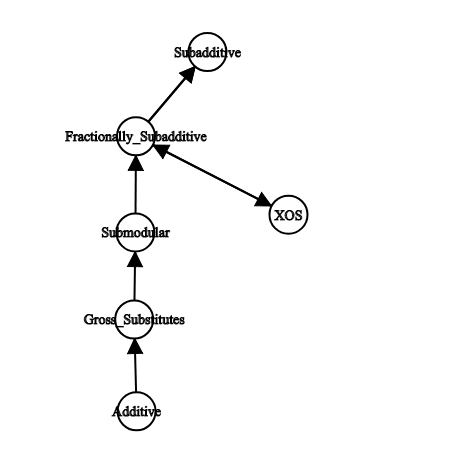
\includegraphics[scale=.8]{graph.png}
\end{center}
Throughout this course, unless explicitly stated otherwise, valuation functions will always be monotone. Each of the other definitions form a hierarchy of valuation functions (see exercises). The first part of this course will focus on various algorithms (ignoring incentives) for welfare maximization in the various models for various classes of valuation functions. This class, we'll see the first algorithm in this series.

\section{A 2-approximation for submodular valuations with value queries}
Lehmann, Lehmann and Nisan consider the following algorithm ~\cite{LehmannLN01}. 
\begin{itemize}
\item Initialize $S_i = \emptyset$ for all $i$.
\item For $j = 1$ to $m$:
\begin{itemize}
\item Query bidder $i$'s value for $M_i(j)= v_i(S_i \cup \{j\})-v_i(S_i)$. 
\item Let $i_j$ denote the bidder with maximum $M_i(j)$.
\item Add item $j$ to $S_i$.
\end{itemize}
\item Output the partition $S_1,\ldots, S_n$.
\end{itemize}

The algorithm is quite simple: it sorts the items arbitrarily, then greedily awards them to whichever bidder has the highest marginal utility for the current item. 

\begin{theorem}[\textrm{[\cite{LehmannLN01}]}]
The algorithm above guarantees a $2$-approximation whenever all $v_i(\cdot)$ are monotone and submodular. The algorithm uses $\poly(n,m)$ value queries.
\end{theorem}
\begin{proof}
The proof proceeds by induction on $m$. Clearly, the algorithm guarantees a $2$-approximation when $m =1$ since it allocates the item optimally. Now, assume for inductive hypothesis that the algorithm guarantees a $2$-approximation for $m$, and we will prove it for $m+1$.

Define $v_{i,j}(S) := v_i(S \cup \{j\}) - v_i(\{j\})$. Consider awarding item $1$ to some bidder $i$ as in the first step of the algorithm, and consider the remaining instance. We make the following observations/steps:
\begin{itemize}
    \item There are only $m$ items left. 
    \item Bidder $i' \neq i$'s value for any additional items $S$ will get them additional value $v_{i'}(S)$, and bidder $i$'s value for additional items $S$ will get them additional value $v_{i,j}(S)$. 
    \item Once we allocate item $1$, it's like we have a new instance where the new valuation functions are the same for all $i' \neq i$ is still $v_{i'}(\cdot)$, and the new $v_i(\cdot) := v_{i,j}(\cdot).$
    \item Continuing our algorithm is \emph{exactly} the same as running our algorithm from scratch on the new valuations.
    \item If we denote by $A_2$ what our algorithm achieves starting from item $2$, and $O_2$ the optimal allocation according to the new values, the inductive hypothesis tells us that $A_2 \geq O_2/2$.\footnote{Actually this claim requires one more fact: that $v_{i,j}(\cdot)$ is submodular. This is proven in the exercises.}
    \item Our algorithm gets welfare exactly $v_i(\{1\}) + A_2$. So our goal is just to show that $OPT \leq O_2 + 2\cdot v_i(\{1\})$, and we'll complete the proof. 
\end{itemize}
To finish the proof, consider the optimal allocation. Some bidder $\ell$ gets item $1$. Now remove item $1$ from $S_\ell$. This partition now only allocates items $\geq 2$, call it $T_1,\ldots, T_n$. First, observe that we must have $\sum_{i' \neq i} v_{i'}(T_{i'}) + v_{i,1}(T_i) \leq O_2$ (by definition of $O_2$ being optimal). Observe also that we have $v_{i,1}(T_i) = v_i(T_i \cup \{1\}) - v_i(\{j\}) \geq v_i(T_i) - v_i(\{1\})$ by monotonicity. Therefore: $\sum_{i'} v_{i'}(T_{i'}) \leq O_2 + v_i(\{1\})$. Moreover, we also have that $v_\ell(T_\ell) + v_\ell(\{1\}) \geq v_\ell(T_\ell \cup \{1\})$ by submodularity (in fact, subadditivity suffices). Therefore we can rewrite OPT as:

$$\sum_{i'} v_{i'}(S_{i'}) = \sum_{i' \neq \ell} v_{i'}(T_{i'}) + v_\ell(T_\ell \cup \{1\}) \leq \sum_{i'} v_{i'}(T_{i'}) + v_{\ell}(\{1\}) \leq O_2 + v_{\ell}(\{1\}) + v_i(\{1\}) \leq O_2 + 2v_i(\{1\}).$$

Where the final step above is because we chose $i$ to receive item $1$ with $v_i(\{1\}) \geq v_\ell(\{1\})$ for all $\ell$. 
\end{proof}

\section{Exercises}
\begin{enumerate}
\item Say that $n=1$. Design a poly-time welfare-maximizing algorithm. Moreover, design a payment rule to make it dominant strategy truthful.
\item Say that $m =1$. Design a poly-time welfare-maximizing algorithm. Moreover, design a payment rule to make it dominant strategy truthful.
\item Say that you are given an algorithm $\mathcal{A}$, which takes as input $n$ valuation functions $v_1,\ldots, v_n$ and outputs a partition maximizing the welfare. Design a dominant strategy truthful mechanism that makes $n+1$ black-box calls to $\mathcal{A}$, and $\poly(n)$ value queries to each $v_i(\cdot)$ and maximizes the welfare (assume that the bidders can indeed ``report'' their valuations without concern for communication/computational constraints).\\
\textbf{Hint:} If you're stuck, Google ``Vickrey-Clarke-Groves.''
\item Prove that every additive function is gross substitutes.
\item Prove that every gross substitutes function is submodular.
\item Prove that every submodular function is fractionally subadditive.
\item Prove that every fractionally subadditive function is subadditive.
\item Prove that XOS and fractionally subadditive are equivalent.\\
 \textbf{Hint:} Find a way to use strong LP duality. If you're stuck, check out~\cite{Feige09}.
\item Prove that the two provided definitions of submodular are equivalent.
\item Prove that $v_{i,j}(\cdot)$ is submodular whenever $v_i(\cdot)$ is submodular (definition as in proof of LLN Theorem). 
\end{enumerate}
\bibliographystyle{alpha}
\bibliography{MasterBib}

\end{document}
